\documentclass[parskip=full]{scrartcl}
\usepackage[T1]{fontenc}    % avoid garbled Unicode text in pdf
\usepackage[utf8]{inputenc} % use utf8 file encoding for TeX sources
\usepackage[german]{babel}  % german hyphenation, quotes, etc
\usepackage{hyperref}       % detailed hyperlink/pdf configuration
\hypersetup{                % ‘texdoc hyperref‘ for options
pdftitle={PSE: Entwicklung eines relationalen Debuggers - Pflichtenheft},%
,%
}
\usepackage{graphicx}       % provides commands for including figures
\usepackage{csquotes}       % provides \enquote{} macro for "quotes"
\usepackage[nonumberlist]{glossaries}     % provides glossary commands
\usepackage{enumitem}
\usepackage{xcolor}
\newcommand\frage[1]{\textcolor{red}{#1}}


\font\myfont=cmr12 at 20pt

\title{
	\vspace{2cm}
	\myfont 
	Praxis der Softwareentwicklung:\\ 
	Entwicklung eines relationalen Debuggers\\
}
\subtitle{
	\vspace{1cm}
	\myfont
	Entwurfsdokument
}
\author{
	\vspace{1cm} \\
	Benedikt Wagner\\
	\texttt{udpto@student.kit.edu}
	\and \vspace{1cm} \\ Chiara Staudenmaier\\
	\texttt{uzhtd@student.kit.edu}
	\and Etienne Brunner\\
	\texttt{urmlp@student.kit.edu}
	\and Joana Plewnia\\
	\texttt{uhfpm@student.kit.edu} 
	\and Pascal Zwick\\
	\texttt{uyqpk@student.kit.edu}
	\and Ulla Scheler\\
	\texttt{ujuhe@student.kit.edu}
	\vspace{1cm}
	\and Betreuer: Mihai Herda, Michael Kirsten
	\vspace{4cm}
}


\begin{document}
\clearpage
\maketitle
\pagenumbering{gobble}
\newpage

\tableofcontents
\newpage
\pagenumbering{arabic}
%Eventuell Fußnoten generieren
\section{Einleitung}
%Einleitung mit grobem Überblick. Dieser Abschnitt soll an das Pflichtenheft anschließen.
Dieses Dokument dokumentiert den Entwurf des Produkts \enquote{DIbugger}, wie es im Pflichtenheft definiert wurde.\\
Hierbei werden das Geheimnisprinzip und Lose Kopplung berücksichtigt, um für erhöhte Verständlichkeit
zu sorgen.
\section{Paketeinteilung} %eventuell fällt jemandem ein besserer Titel ein
%Paketdiagramm, Erläuterung der Einteilungsentscheidung, Schnittstellen
\subsection{Übersicht}

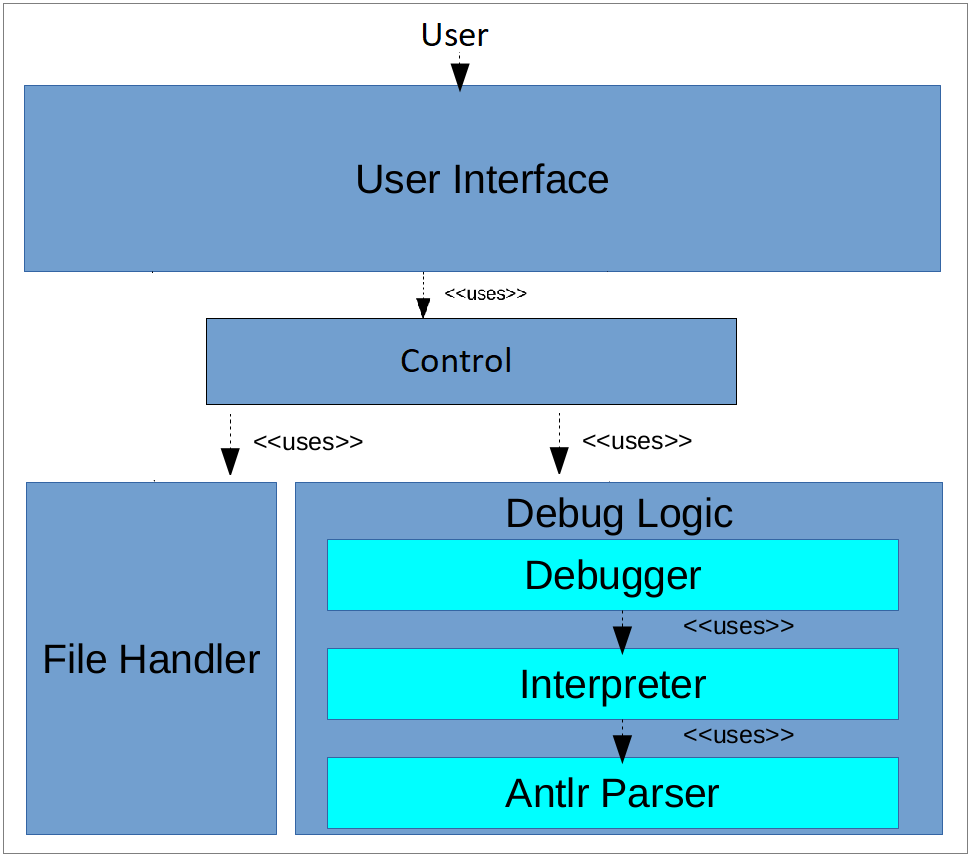
\includegraphics[scale=0.35]{../Plichtenheft/Architektur.png}
Das Produkt ist aufgeteilt in die Pakete \enquote{Control}, \enquote{User Interface}, \enquote{File Handler} und \enquote{Debug Logic}.
Hierbei besteht die Debug Logic aus den Unterpaketen \enquote{Debugger}, \enquote{Interpreter} und
\enquote{Antlr Parser}.

\subsection{Erläuterung der einzelnen Pakete}
\subsubsection{User Interface}
\paragraph{Aufgaben}
\paragraph{Schnittstellen}
\paragraph{Benutztrelation} z.B. 1 benutzt 2, weil (durch, indem ...)
\subsubsection{Control}
\paragraph{Aufgaben}
\paragraph{Schnittstellen}
\paragraph{Benutztrelation}
\subsubsection{File Handler}
\paragraph{Aufgaben}
\paragraph{Schnittstellen} Eventuell aufteilen in benötigte und angebotene?
\paragraph{Benutztrelation} 
\subsubsection{Debug Logic}
Paket ist ein verdammt seltsames Wort: Paket, Paket
\paragraph{Debugger}
\subparagraph{Aufgaben}
\subparagraph{Schnittstellen}
\subparagraph{Benutztrelation} 
\paragraph{Trace Generator}
\subparagraph{Aufgaben}
\subparagraph{Schnittstellen}
\subparagraph{Benutztrelation} 
\paragraph{Relational Expression Generator}
\subparagraph{Aufgaben}
\subparagraph{Schnittstellen}
\subparagraph{Benutztrelation} 
\paragraph{Antlr Parser}
\subparagraph{Aufgaben}
\subparagraph{Schnittstellen}
\subparagraph{Benutztrelation} 

\section{Beschreibung der Klassen}
Detaillierte Beschreibung aller Klassen. Das beinhaltet (JavaDoc) Beschreibungen zu allen Me-
thoden, Konstruktoren, Packages und Klassen. Was hier nicht reingehört sind private Felder
und Methoden. Das sind Implementierungsdetails.

\subsection{Klassen in Paket 1}
\subsection{Klassen in Paket 2} 
...

\section{Charakteristische Abläufe}
Beschreibung von charakteristischen Abläufen anhand von Sequenzdiagrammen. Beispielswei-
se bieten sich Testszenarien aus dem Pflichtenheft hier an. Wir empfehlen Sequenzdiagramme
möglichst früh zu erstellen, denn dabei werden die Schnittstellen zwischen Packages und Klas-
sen klar. 
Auf Klassen oder Pakete in Beschreibung aller Klassen verweisen


\section{Abhängigkeitseinteilung}
Mit Blick auf den Implementierungsplan: Aufteilung in Klassen/Pakete, die unabhängig vonein-
ander implementiert und getestet werden können.

\section{Formale Spezifikation von Kernkomponenten}
Speicherformate, Sprachdefinition(formal)

\section{Änderung zum Pflichtenheft}
Änderungen zum Pflichtenheft, z.B. gekürzte Wunschkriterien.




\section{Anhang}
UML-Klassendiagramm 
Vollständiges großformatiges Klassendiagramm im Anhang. Ausschnitte/Teile können bereits
vorher verwendet werden, um Teilkomponenten zu beschreiben. Assoziationen zwischen Klas-
sen dabei bitte mit entsprechenden Pfeilen darstellen, statt nur durch Feldtypen.
Identifikation von Entwurfsmustern um Struktur gröber zu beschreiben.





\end{document}
\grid
